\iftoggle{icmlworkshop}{
\section{Analysis: IO Complexity of \sysname}
}
\subsection{Analysis: IO Complexity of \sysname}
\label{sec:theory}

We analyze the IO complexity of \sysname, showing
significant reduction in HBM accesses compared to standard attention.
We also provide a lower bound, proving that no exact attention algorithm can asymptotically improve on HBM accesses over all
SRAM sizes.
Proofs are in \cref{sec:proofs}.

\begin{theorem}\label{thm:io_complexity}
  Let $N$ be the sequence length, $d$ be the head dimension, and $M$ be size of
  SRAM with $d \leq M \leq Nd$.
  Standard attention (\cref{alg:standard_attn}) requires $\Theta(Nd + N^2)$ HBM
  accesses, while \sysname (\cref{alg:stream_attn}) requires
  $\Theta ( N^2 d^2 M^{-1} )$ HBM accesses.
\end{theorem}
For typical values of $d$ (64-128) and $M$ (around 100KB), $d^2$ is many
times smaller than $M$, and thus \sysname requires many times fewer
HBM accesses than standard implementation.
This leads to both faster execution and lower memory footprint, which we
validate in~\cref{sec:benchmark}.

The main idea of the proof is that given the SRAM size of $M$, we
can load blocks of $\vK, \vV$ of size $\Theta(M)$ each (\cref{alg:stream_attn} line \ref{alg:stream_attn_load_kv}).
For each block of $\vK$ and $\vV$, we iterate over all blocks of $\vQ$
(\cref{alg:stream_attn} line \ref{alg:stream_attn_load_qo}) to compute the
intermediate values, resulting in $\Theta(NdM^{-1})$ passes over $\vQ$.
Each pass loads $\Theta(Nd)$ elements, which amounts to $\Theta(N^2 d^2 M^{-1})$ HBM accesses.
We similarly prove that the backward pass of standard attention requires
$\Theta(Nd + N^2)$ HBM accesses while the backward pass of \sysname requires
$\Theta(N^2 d^2 M^{-1})$ HBM accesses (\cref{sec:algo_details}).

We prove a lower-bound: one cannot asymptotically improve on the number of HBM
accesses for all values of $M$ (the SRAM size) when computing exact attention.
\begin{proposition}\label{thm:lower_bound}
  Let $N$ be the sequence length, $d$ be the head dimension, and $M$ be size of
  SRAM with $d \leq M \leq Nd$.
  There does not exist an algorithm to compute exact attention with
  $o(N^2d^2 M^{-1})$ HBM accesses for all $M$ in the range
  $[d, Nd]$.
\end{proposition}
The proof relies on the fact that for $M = \Theta(Nd)$ any algorithm must perform
$\Omega ( N^2d^2M^{-1} ) = \Omega(Nd)$ HBM accesses.
This type of lower bound over a subrange of $M$ is common in the streaming
algorithms literature~\citep{woodruff2004optimal}.
We leave proving parameterized complexity~\citep{flum2006parameterized} lower
bounds in terms of $M$ as exciting future work.

We validate that the number of HBM accesses is the main determining factor of
attention run-time.
In~\cref{fig:micros} (left), we see that even though \sysname has
higher FLOP count compared to standard attention (due to recomputation in the
backward pass), it has much fewer HBM accesses, resulting in much faster
runtime.
In~\cref{fig:micros} (middle), we vary the block size $B_c$ of \sysname, which results in different amounts of HBM accesses, and measure the
runtime of the forward pass.
As block size increases, the number of HBM accesses decreases (as we make fewer
passes over the input), and runtime decreases.
For large enough block size (beyond 256), the runtime is then bottlenecked by
other factors (e.g., arithmetic operations).
Moreover, larger block size will not fit into the small SRAM size.

\begin{figure}[t]
  \captionsetup{font=small}
    \centering
    \begin{minipage}{2.3in}
        \centering
        \resizebox{0.98\linewidth}{!}
        {
        \begin{tabular}{@{}c|ccc@{}}
          Attention & Standard & \sysname \\ \hline
          GFLOPs & 66.6 & 75.2 \\
          HBM R/W (GB) & 40.3 & 4.4 \\
          Runtime (ms) & 41.7 & 7.3
        \end{tabular}
        }
    \end{minipage}
    \begin{minipage}{3in}
        \centering
        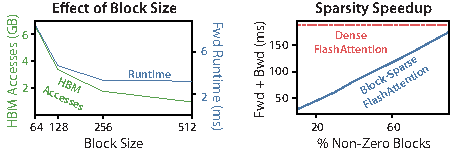
\includegraphics[width=3in]{figs/flashattn_micros.pdf}
    \end{minipage}
    \captionsetup{font=small}
    \caption{\label{fig:micros}
    \textbf{Left}: Forward + backward runtime of
    standard attention and \sysname for GPT-2 medium
    (seq.\ length 1024, head dim.\ 64, 16 heads, batch size 64) on
    A100 GPU.
    HBM access is the primary factor affecting runtime.
    \textbf{Middle}: Forward runtime of \sysname
    (seq.\ length 1024, head
    dim.\ 64, 16 heads, batch size 64)
    on A100 GPU. Fewer HBM accesses result in faster runtime, up to a point.
    \textbf{Right}: The runtime (for seq.\ length 4K) of
  block-sparse \sysname is faster than \sysname by a factor proportional
  to the sparsity.
    }
    \vspace{-1.0em}
\end{figure}



